\section{Introduction}
\label{sec:introduction}

\par The main objective od this laboratory assignment is to produce an AC/DC converter using a transformer, an envelope detector and a voltage regulator, in order to convert the AC input voltage, whose amplitude and frequency were given to us, into a DC output voltage of 12V. To achieve this objective affectively, two factors had to be taken into consideration, the voltage ripple and the cost of the circuit. The relationship between these two factors produces the Merit \ref{eq:merit}, whose value we want to be as high as possible. 

\begin{equation}
  M = \frac {1}{cost*(ripple(v_{o}) + average(v_{o} - 12) + 10^{-6})}.
  \label{eq:merit}
\end{equation}


\par The circuit used to convert the signal is shown in Figure\ref{fig:circuit}.

\begin{figure}[h] \centering
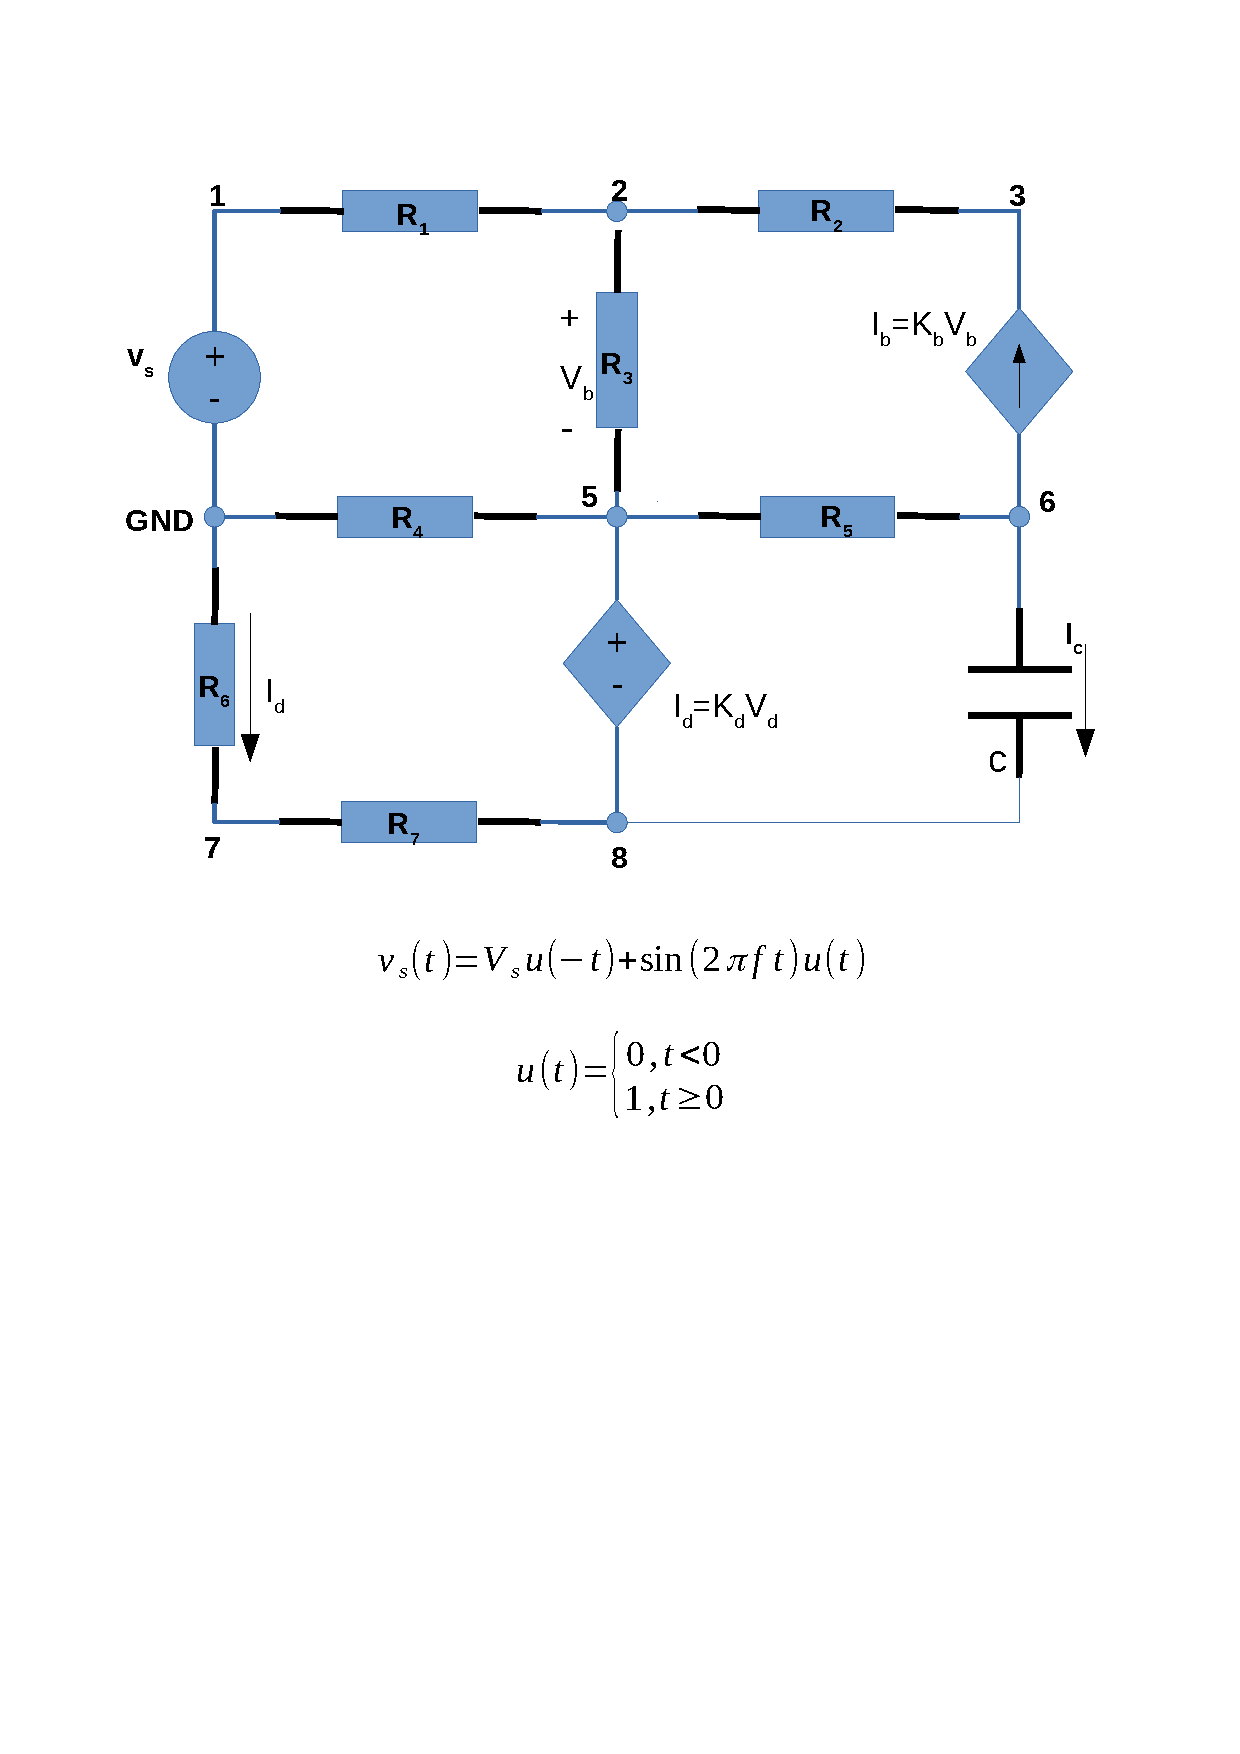
\includegraphics[width=0.6\linewidth]{circuit.pdf}
\caption{Circuit under analysis.}
\label{fig:circuit}
\end{figure}


\par In the next section (~\ref{sec:analysis}), we briefly explain the procedure to analyse theoretically the circuit above with the use of Octave maths tool. In Section 3 a simulation analysis is given, where we resorted to Ngspice to simulate the circuit, and a few graphics are presented to understand the results. The report finishes with its conclusion in section~\ref{sec:conclusion}, where we analyse side by side the theoretical and simulated results and resume the most important points of the lab assignment.

\newpage
